\documentclass[12pt,titlepage,german,a4]{article}

\usepackage{graphicx}
\hyphenation{Speicher-zel-le}

\renewcommand{\contentsname}{Inhaltsverzeichnis}

\begin{document}
    \title{\bf Miniprojekt: Minimax-Maschine \\ Pflichtenheft}
    \date{Hardware Projekt 2017 \\ 03. Januar 2017}
    \author{Maximilian Lumpe, Niklas Blume, Jan Feuchter, Phu Bac Duong}
    \maketitle

    \tableofcontents

    \newpage

    \section{Einleitung}
    In diesem Miniprojekt im Rahmen des Hardware-Praktikums besch{\"a}ftigen wir uns mit der Minimax-Maschine, welche uns grundlegend aus der Vorlesung "Grundlagen der Rechnerarchitektur" bekannt ist. Zur L{\"o}sung der Aufgaben ist es hierbei notwendig, die vorgegebene Grundstruktur der Maschine geeignet zu erweitern, um die Algorithmen zu realisieren.\\Die Vorbereitung auf unser Projekt wird dokumentiert und strukturiert durch das von uns erstellte Pflichtenheft. Das Pflichtenheft wird nur unsere Vorbereitung beinhalten. Die Ergebnisse werden in einer weiteren Dokumentation enthalten sein.

    \section{Aufgabe: Paketanalyse}
    Nach unserem Verst{\"a}ndnis ist das Ziel der Aufgabenstellung das Implementieren des Algorithmus "Paketanalyse" auf der Minimax-Maschine. Dieser Algorithmus wertet die L{\"a}nge des Nutzdatenteils der Datenpakete aus dem Speicher der Maschine aus.\\Jedes Paket besteht aus einem Header mit 80 Bits, gefolgt von dem Datenteil mit variabler L{\"a}nge. Ein Paket beginnt mit dem festgelegten Bitmuster 1110. Der Header enth{\"a}lt eine 2 Bytes lange Kanalnummer, die bei der Bitstelle 32. beginnt. Zu einem Kanal geh{\"o}ren mehrere Datenpakete mit einer eindeutigen Kanalnummer. Die Anzahl der Bits, die in den Speicher geladen werden, wird als bekannt vorausgesetzt und wird in ein entsprechendes Register vorgeladen.\\Nun soll der "Paketanalyse"-Algorithmus eine Tabelle, die Kanalnummern und zugeh{\"o}rige Datenl{\"a}ngen (in Bits) enth{\"a}lt, anlegen. Haben mehrere Pakete dieselbe Kanalnummer, so werden die L{\"a}ngen des Nutzdatenteils addiert. Die Tabelle soll ab einer beliebigen Speicheradresse au{\ss}erhalb des Paketfeldbereichs im Hauptspeicher der Maschine abgelegt werden.\\Diese Aufgabenstellung soll mit dem gegebenen Minimax-Simulator simuliert und getestet werden. Die Maschine kann durch vorgegebene Bauteile erweitert werden, was sich jedoch auf die Bewertung auswirkt. Der Algorithmus wird in Form der Steuertabelle implementiert und soll au{\ss}erdem als Flussdiagramm abgegeben werden.

    \newpage

    \section{Ist-Analyse der Basismaschine}
    Im Rahmen der Vorlesung "Grundlagen der Rechnerarchitektur" haben wir die Minimax-Maschine als Beispiel kennengelernt. Diese Minimax-Maschine ist ein Rechensystem, welches auf dem Grundprinzip der Von-Neumann-Architektur  basiert. Im Wesentlichen  besteht das System aus einigen Registern und einer arithmetisch-logischen Einheit (ALU), welche den Datenpfad bilden, und einem Hauptspeicher (HS), in welchem Code und Daten gemeinsam liegen.

    \subsection{Register der Basismaschine}
    Die Basismaschine besteht zun{\"a}chst nur aus f{\"u}nf Registern, welche f{\"u}r Grundfunktionen der Maschine ben{\"o}tigt werden. Diese sind ACCU (zum Speichern von Ergebnissen der ALU), PC (zum Speichern der Nummer der aktuellen Programmzeile), MDR (zum Speichern von aus dem HS gelesenen Daten), IR (zum Speichern des Befehls der aktuellen Programmzeile) und MAR (zum Anlegen bestimmter Speicheradressen).\\
    Die Register sind als zweiflankengesteuerte Master-Slave-Flipflops ausgelegt. Damit kann ein Register w{\"a}hrend eines Taktimpulses zun{\"a}chst als Quelle und dann als Ziel dienen. Der Befehlsablauf dieses Systems wird {\"u}ber ein Mikroprogramm festgelegt. F{\"u}r unser Projekt kann die Architektur der Minimax-Maschine um zus{\"a}tzliche Register erweitert werden.


    \subsection{Operationen der ALU}
    In der Basismaschine kann die ALU zun{\"a}chst nur vier Operationen ausf{\"u}hren (bezeichnet mit:  ADD, SUB, TRANS.A, TRANS.B). Die ALU kann aber durch zus{\"a}tzliche Operationen, wie z.B. dem DIV-Befehl, erg{\"a}nzt werden.
    \begin{itemize}
        \item ADD: Addiert zwei Register
        \item SUB: Subtrahiert zwei Register
        \item TRANS.A: Leitet den Wert A durch
        \item TRANS.B: Leitet den Wert B durch
    \end{itemize}
    Das Ergebnis kann an eines der oben genannten Register geleitet werden. \\
    \begin{table}[htpb]
        \centering
        \label{hi}
        \begin{tabular}{ccc}
            Symbol & ALU-Operation & ALU Ctrl \\
            \hline
            ADD & ALUresult \leftarrow A + B & 00 \\
            SUB & ALUresult \leftarrow -A + B & 01 \\
            Trans.A & ALUresult \leftarrow A & 10 \\
            Trans.B & ALUresult \leftarrow B & 11
        \end{tabular}
        \caption{ALU-Operationen der Basisimaschine}
    \end{table}

    \subsection{Ein- und Ausgabewerte der ALU}
    Die Eingangswerte A und B der ALU k{\"o}nnen {\"u}ber zwei Multiplexer bestimmt werden. A kann die Werte 0, 1 und ACCU annehmen, B die Werte MDR, PC, IR und ACCU. \\
    Das Ergebnis einer Operation wird als ALU-result auf einen Bus gegeben, wodurch es an jedes beliebige Register geleitet werden kann. Eine weiter Datenleitung f{\"u}hrt zur CU, wodurch bestimmte Flags gesetzt werden k{\"o}nnen(z.B. wenn das Ergebnis der Operation 0 ist)

    \subsection{CPU-Befehle}
    Die CPU-Befehle sind 32 Bit breit, wobei das h{\"o}chstwertige Byte immer den Opcode enth{\"a}lt. Die verbleibenden 3 Bytes bestimmen dann den Adressteil. Der Opcode und die Operanden werden zun{\"a}chst vollst{\"a}ndig aus dem Hauptspeicher geladen, bevor ein Befehl ausgef{\"u}hrt wird.

    \newpage

    \section{Beschreibung des Implementierungskonzeptes}
    Bei der Implementierung der Paketanalyse muss zwischen mehreren Teilschritten unterschieden werden. Zun{\"a}chst wird nach dem Startbitmuster des ersten Paketes gesucht (1). Ist ein Paket identifiziert, k{\"o}nnen die ersten 32 Bits (dies entspricht einer Speicherzelle) {\"u}bersprungen werden. Somit beginnt mit der zweiten Speicherzelle die Kanalnummer des Paketes, diese wird extrahiert und abgespeichert (2). Nach 32 weiteren Bits kommt nun der Datenteil, welcher Bit f{\"u}r Bit ausgelesen wird, w{\"a}hrend gleichzeitig ein Z{\"a}hlregister inkrementiert wird (3). W{\"a}hrend dieses Vorgangs wird permanent {\"u}berpr{\"u}ft, ob ein neues Startbitmuster vorliegt, sodass ein neues Paket anf{\"a}ngt (4). Ist dies der Fall, wird das Z{\"a}hlregister auf den momentanen Wert f{\"u}r die Kanalnummer addiert. Die Kanalnummer dient dabei als Offset f{\"u}r die Speicherzelle (5).

    \subsection{Identifizierung des Startbitmusters}
    Da f{\"u}r das Startbitmuster nur die vier niedrigwertigsten Bits untersucht werden, m{\"u}ssen zun{\"a}chst f{\"u}r einen Vergleich die restlichen ausgeblendet werden. Dies erfolgt durch eine bitwise-and Verkn{\"u}pfung mit Nullen. Anschlie{\ss}end wird das Ergebnis mit dem Startbitmuster verglichen. Sind sie nicht identisch, wird die Speicherzelle geshiftet. Dies wird solange wiederholt, bis das Ergebnis identisch ist, dann wird mit Schritt 2 fortgefahren.

    \subsection{Kanalnummer extrahieren}
    In der ersten Speicherzelle stehen nun die 4 Bits des Startmusters, sowie 28 Bits die {\"u}bersprungen werden. Also enth{\"a}lt die erste Speicherzelle keine weiteren Informationen, sodass mit der n{\"a}chsten Speicherzelle fortgefahren wird. Nun m{\"u}ssen die ersten 16 Bits, die die Kanalnummer beinhalten, extrahiert werden. Hierf{\"u}r sorgt wieder die bitwise-and Verkn{\"u}pfung der restlichen Bits mit Nullen. Die Kanalnummer muss f{\"u}r die sp{\"a}tere Nutzung abgespeichert werden.

    \subsection{Datenbits z{\"a}hlen}
    Auch die zweite Speicherzelle enth{\"a}lt nun keine Informationen mehr. Da in der dritten Speicherzelle noch 16 Bits sind, die nicht zum Datenteil geh{\"o}ren, werden im ersten Durchlauf nur 16 auf das Z{\"a}hlregister f{\"u}r die L{\"a}nge des Datenteils addiert. F{\"u}r jeden weiteren Schleifendurchlauf werden dann 32 addiert.

    \subsection{Auf neues Startbitmuster {\"u}berpr{\"u}fen}
    W{\"a}hrend die Datenbits nach und nach durch shiften gez{\"a}hlt werden, wird permanent auch der Test aus (1) durchgef{\"u}hrt. Sobald das Startbitmuster erkannt ist, bricht die Schleife aus (3) ab und es folgt Schritt (5).

    \subsection{Z{\"a}hlregister zur Tabelle hinzuf{\"u}gen}
    Um die Tabelle zur Speicherung der L{\"a}ngen von den eigentlichen Daten zu trennen, darf diese erst in einer Speicherzelle nach der maximalen Datenl{\"a}nge beginnen. Ab dieser Speicherzelle repr{\"a}sentieren immer zwei aufeinanderfolgende Speicherzellen eine Reihe dieser Tabelle. So beinhaltet die erste Speicherzelle die Kanalnummer 0, die zweite Speicherzelle den entsprechenden Wert f{\"u}r diesen Kanal. Die dritte Speicherzelle beinhaltet wieder die Kanalnummer der n{\"a}chsten Zeile, in diesem Fall die Nummer 1. Danach kommt wieder der Wert f{\"u}r Kanal 1 und so weiter. Die Adresse der ersten Speicherzelle f{\"u}r die Adresse soll dabei in einem Register gespeichert sein. Nun wird die doppelte Kanalnummer auf dieses Register addiert, um die Speicherzelle f{\"u}r eine bestimmte Kanalnummer zu erhalten. Eine Speicherzelle weiter ist somit der entsprechende Wert. Auf den Inhalt dieser Speicherzelle wird dann der Inhalt des Z{\"a}hlregisters addiert. Anschlie{\ss}end werden die tempor{\"a}ren Register zur{\"u}ckgesetzt und der Algorithmus beginnt erneut mit Schritt (2).

    \newpage

    \section{Angestrebte Projektergebnisse}
        \begin{itemize}
			\item Ein Pflichtenheft, in dem wir unsere Vor{\"u}berlegungen festhalten.
			\item Eine vollst{\"a}ndige und funktionsf{\"a}hige L{\"o}sung mit allen Testdateien.
			\item Einen Schaltplan, bei dem wir die gegebene Minimax-Maschine um die notwendigen Elemente erweitert haben.
			\item Eine vollst{\"a}ndige Dokumentation, mit der wir unseren Algortihmus und unsere implementierte L{\"o}sung beschreiben und erl{\"a}utern.
        \end{itemize}

	\section{Arbeitsaufteilung}
		\begin{itemize}
			\item Maximilian Lumpe: Einleitung und Aufgabenstellung
			\item Phu Bac Duoung: Ist-Analyse der Basismaschine
			\item Jan Feuchter: Beschreibung des Implementierungskonzeptes
			\item Niklas Blume: Angestrebte Projektergebnisse und Anhang
		\end{itemize}

    \newpage

    \section{Anhang: Flussdiagramme geplanter Mikroprogramme}

	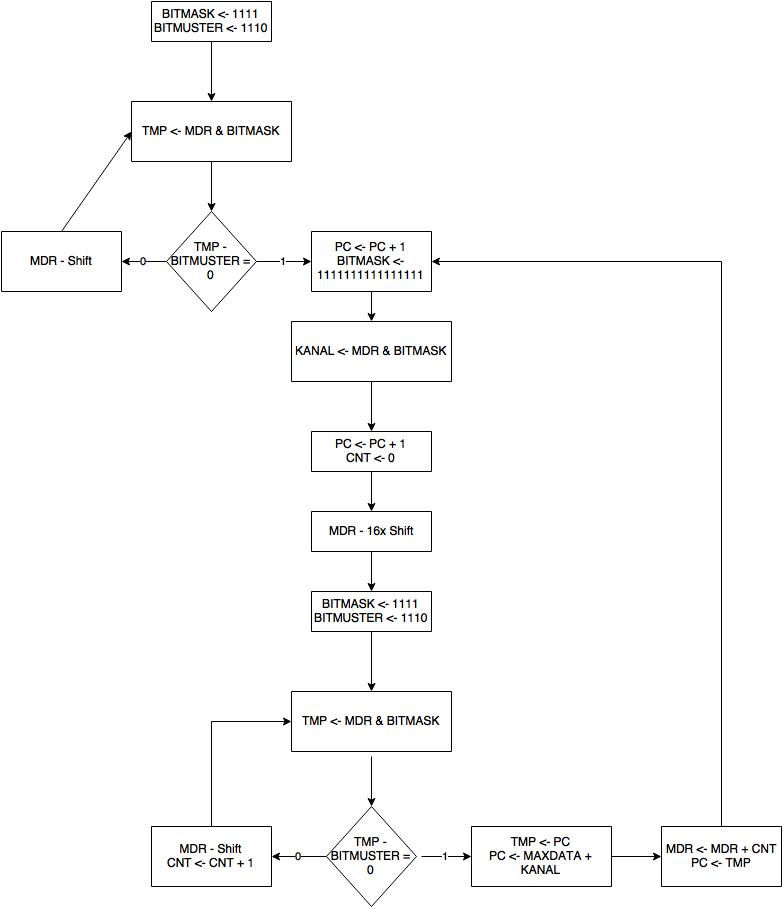
\includegraphics[width=13cm]{algoComplete.png}

	\newpage
    \section{Anhang: Verwendete Hilfsmittel}
	\begin{itemize}
		\item Vorlesung: Grundlagen der Rechnerarchitektur
		\item Umdruck Paketanalyse 2016/17
		\item GitHub zur Versionskontrolle und Organisation
		\item \url{https://www.draw.io} zur Erstellung der Flussdiagramme
	\end{itemize}


\end{document}
